\documentclass[12pt]{article} % Default font size is 12pt, it can be changed here

\usepackage[utf8]{inputenc} % utf8 encoding
\usepackage{geometry} % Required to change the page size to A4
\geometry{a4paper} % Set the page size to be A4 as opposed to the default US Letter

\usepackage{graphicx} % Required for including pictures
\usepackage{float} % Allows putting an [H] in \begin{figure} to specify the exact location of the figure

\linespread{1.2} % Line spacing

%\setlength\parindent{0pt} % Uncomment to remove all indentation from paragraphs

\graphicspath{{pictures/}} % Specifies the directory where pictures are stored

\usepackage{listings} % To be able to have code in text
\usepackage{color} % To be able to have colors

\definecolor{codegreen}{rgb}{0,0.6,0}
\definecolor{codegray}{rgb}{0.5,0.5,0.5}
\definecolor{codepurple}{rgb}{0.58,0,0.82}
\definecolor{backcolour}{rgb}{0.95,0.95,0.92}
 
\lstdefinestyle{codestyle}{
    backgroundcolor=\color{backcolour},   
    commentstyle=\color{codegreen},
    keywordstyle=\color{magenta},
    numberstyle=\tiny\color{codegray},
    stringstyle=\color{codepurple},
    basicstyle=\footnotesize,
    breakatwhitespace=false,         
    breaklines=true,                 
    captionpos=b,                    
    keepspaces=true,                 
    numbers=left,                    
    numbersep=5pt,                  
    showspaces=false,                
    showstringspaces=false,
    showtabs=false,                  
    tabsize=2
}
 
\lstset{style=codestyle}

\begin{document}

%----------------------------------------------------------------------------------------
%   TITLE PAGE
%----------------------------------------------------------------------------------------

\begin{titlepage}

\newcommand{\HRule}{\rule{\linewidth}{0.5mm}} % Defines a new command for the horizontal lines, change thickness here

\center % Center everything on the page

\textsc{\LARGE Lund University, Faculty of Engineering}\\[1.5cm] % Name of your university/college
\textsc{\Large EDAA40}\\[0.5cm] % Major heading such as course name
\textsc{\large Discrete Strucures in Computer Science}\\[0.5cm] % Minor heading such as course title

\HRule \\[1cm]
{ \huge \bfseries Summary of EDAA40}\\[0.4cm] % Title of your document
\HRule \\[1.5cm]

\emph{Author:} Fred \textsc{Nordell} % Your name

{\large \today}\\[3cm] % Date, change the \today to a set date if you want to be precise

%\includegraphics{Logo}\\[1cm] % Include a department/university logo - this will require the graphicx package

\vfill % Fill the rest of the page with whitespace

\end{titlepage}

%----------------------------------------------------------------------------------------
%   TABLE OF CONTENTS
%----------------------------------------------------------------------------------------

\tableofcontents % Include a table of contents
\lstlistoflistings % Include a table of lstlistings
\listoffigures % Include listing of figures
\listoftables

\newpage % Begins the essay on a new page instead of on the same page as the table of contents 


\section{Sets} % Major section

Sets are collections of stuff, any stuff. There is one special set, the empty set: $\{\} = \emptyset$. Given a set A, any ting x is either an element of A or it is not; $x \in A$ or $x \notin A$. To make this work we need a concept of equality, is $\{2,1\} \in \{\{1,2\},\{3,4\}\}$ ? 

\subsection{Extensionallity}
A set is defined by the elements it contains (its \textit{extension}). Order and repetition does not matter. $\{a,b,c\} = \{c,b,a\} = \{a,a,b,c,b\}$ Equal sets must contain \textit{exactly} the same elements $\{a,b,c\} \neq \{a,c,b,d\}$. Note that 1-element sets are \textit{singleton} sets: $\{a,b,c\} \neq \{\{a,b,c\}\}$ \& $\emptyset \neq \{\emptyset\}$ \& $11 \neq \{11\}$.

\subsection{Cardinallity}

The number of elements in a set $A$ is called its cardinallity. $\#(A)$ or $|A|$. Note that $\#(\emptyset) = 0$

\subsection{Inclusion}
If $A \subseteq B$ we call A a \textit{subset} of B and B the \textit{superset} of A. This means that if $x \in A$ then $x \in B$. A and B might be the same, in fact: $A \subseteq B$ and $B \subseteq A$ iff (if and only if) $A = B$. Furthermore, for any set A it is allways the case that $\emptyset \subseteq A$ and $A \subseteq A$. Note that $\subset$ is used to denote \textit{proper} inclusion: $A \subset B$ iff $A \subseteq B$ and $A \neq B$.

\subsubsection{Properties of inclusion}
Inclusion is \textit{transitive}: $A \subseteq B$ and $B \subseteq C$ implies $A \subseteq C$. Inclusion is also \textit{partial}: There are sets where neither $A \subseteq B$ or $B \subseteq A$ is true.

\subsection{Specifying sets}
There are a couple of ways to define sets: enumeration, set builder and recursive defenition.

\subsubsection{Enumeration}
Simple, just list the elements: $A = \{2,3,4,5,7,11\}$

\subsubsection{Builder notaion}
Little more complicated: $B = \{x \in A: x \quad odd\} \rightarrow B = \{3,5,7,11\}$. This uses other sets to select different elements based on a condidtion. 

\par Here we find \textit{Russel's paradox}, that is $R = \{x: x\notin x\}$ but does $R \in R$? Here $R$ isn't a well-defined set, $x$ can stand for anything, even things that aren't a set. Because of this we make sure that varibles are limited to elements of a set that is known to be well-defined. This form automatically implies a superset.

\subsubsection{Recursive}

\subsection{Operations on sets}
\subsubsection{Union}
The union, $A \cup B$,of $A$ and $B$ is all elements that are in $A$ or $B$. That is: $x \in A \cup B$ iff $x \in A$ or $x \in B$

\subsubsection{intersection}
The intersection, $A \cap B$, of $A$ and $B$ is all elements that are both in $A$ and $B$. That is: $x \in A \cap B$ iff $x \in A$ and $x \in B$.

\subsubsection{difference}
The difference, $A \setminus B$, of $A$ and $B$ is all elements that are in $A$ and not in $B$. That is: $x \in A \setminus B$ iff $x \in A$ and $x \notin B$.

\begin{figure}[H]
\center{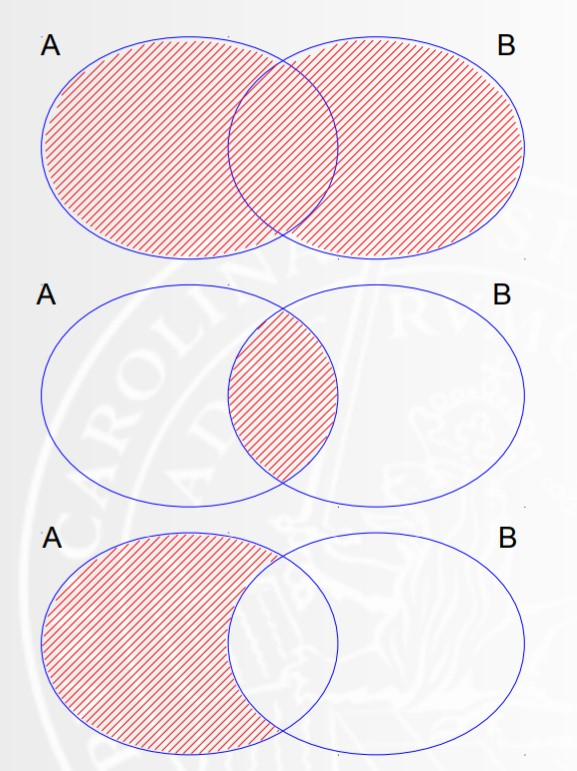
\includegraphics[width=0.5\linewidth]{operation.jpg}}
\caption{Illustration of set operations}
\label{operations}
\end{figure}

\subsubsection{Complement}
There is no general \"inverse\" set $-A$ for the set $A$. However we often work in a \textit{local universe}, that is a set of everything we are potentionally interested in. Let's call it $U$. We can con give the complement of a set a meaning: $-A = U \setminus A$. Can also be written $A^- \quad A' \quad A^c$

\subsection{Disjointness}
Two sets are \textit{disjoint} if they do not share any common elements: $A \cap B = \emptyset$. All sets are disjoint from $\emptyset$, event the empty set. For multiple sets they are \textit{pairwise disjoint} if they are all disjoint.

\subsection{Algebra}

\begin{figure}[H]
\center{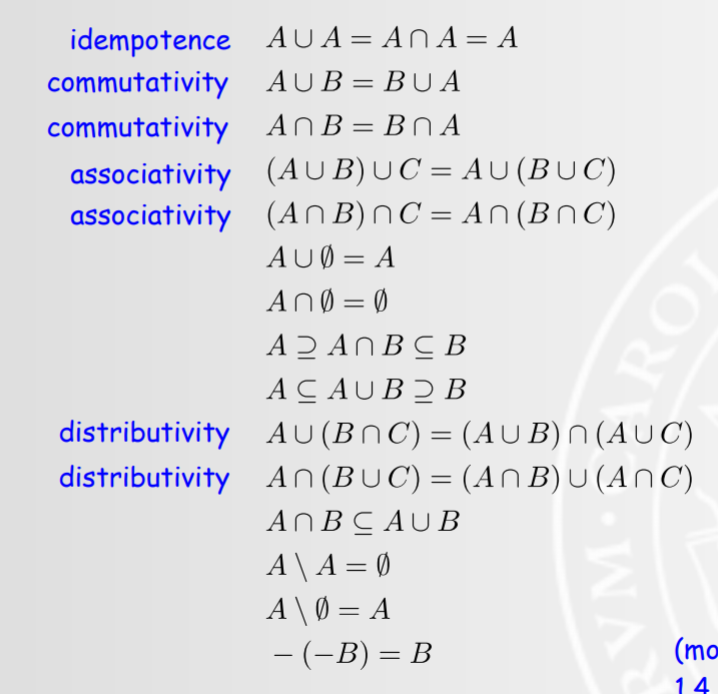
\includegraphics[width=0.5\linewidth]{algebra.png}}
\caption{Illustration of set algebra}
\label{set algebra}
\end{figure}

\subsection{Set families}

A family of sets is a way of reffering to a set of sets, usually \textit{indexed} by an \textit{index set}. $\{A_i : i \in I\}$, where $A_i$ are sets, $i$ is the index and $I$ is the index set.

\subsubsection{Generalized union and intersection}
Let $S$ be a set of sets then $\bigcap S = \{x : x \in s$ for all $s \in S\}$ and $\bigcup S = \{ x : x \in s$ for at least one $s \in S\}$

\subsection{Power sets}

The \textit{power set} of a set A is the set of all its subsets. $\mathcal{P}(A) = \{s : s \subseteq A \} = 2^A$

\begin{itemize}
    \item $\mathcal{P}(\emptyset) = \emptyset$
    \item $\mathcal{P}(\{a\}) = \{\emptyset, \{a\}\} $
    \item $\mathcal{P}(\{a,b\}) = \{\emptyset, \{a\}, \{b\}, \{a,b\}\}$
    \item $\mathcal{P}(\{a,b,c\}) = \{\emptyset, \{a\},\{b\},\{c\},\{a,b\},\{a,c\},\{b,c\},\{a,b,c\}\}$
    \item $\#(\mathcal{P}(A)) = 2^{\#(A)}$ 
\end{itemize}

\begin{figure}[H]
\center{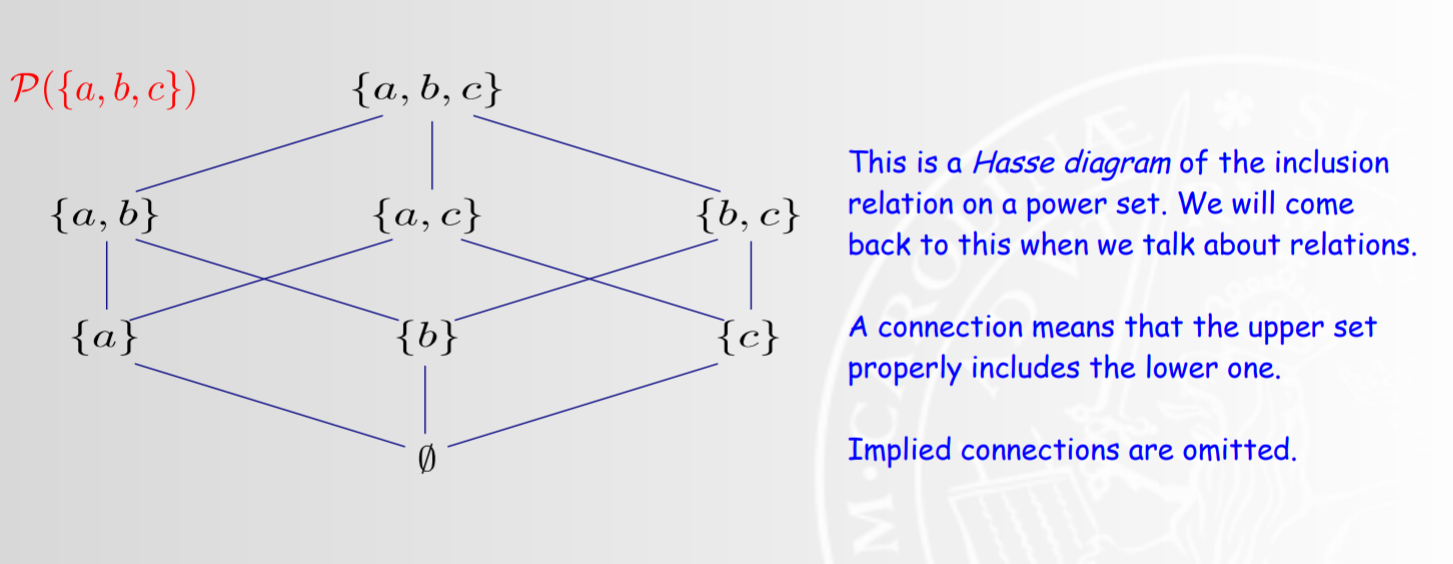
\includegraphics[width=0.5\linewidth]{hasse.png}}
\caption{Hasse diagram of powerset}
\label{hasse diagram}
\end{figure}

\section{Relations}

Mathematical relation are about connections between objects. It can be relations between numbers: a divides b, a is greater than etc. or it can be relations between sets: A is a subset of B, same size etc. or it can be between people: customer/client, parent/child.

\subsection{Ordered pairs}
An ordered pair is diffeent from an unordered pair wich we have seen before in that the flipped pair is not the same. $(a,b) = (x,y)$ iff $a = x$ and $b = y$, corollary: $(a,b) \neq (b,a)$ if $a \neq b$. N-tuples is this idea but with n number of elements in the tulple.

\subsection{Cartesian product}
The cartesian product of a pair of sets, or generally a finite family of sets, is the set of all ordered pais or n-tuples.
\[
    A_1 \times ... \times A_n = \{(a_1 , ...,a_n) : a_1 \in A_1, ..., a_n \in A_n\}
\]
If sets are the same we also write $A \times A = A^2$

\begin{figure}[H]
\center{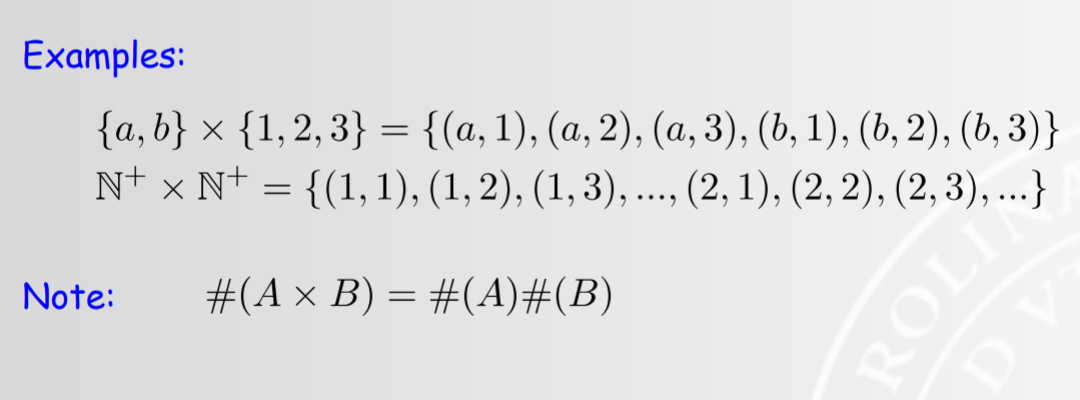
\includegraphics[width=0.5\linewidth]{cartesian.png}}
\caption{Examples of cartesian product}
\label{Cartesian product examples}
\end{figure}

\subsection{Relation and natural join}

A (binary, dyadic) relation R from A to B, or over $A \times B$, is a subset of the cartesian product.

\[
    R \subseteq A \times B
\]

If A and B are the same i.e. $R \subseteq A \times A$ we call R a binary relation over A. For binary relations $R \subseteq A \times B$, these are equvalent: $(a,b) \in R$ and $aRb$. The $\bowtie$ operator is the \textit{natural join}, that gives the set of all combinations of tuples in the relations, $R \bowtie S$, taht are equal on their commn attribute names. It is important because it is the relational counterpart to the logical AND.

\begin{figure}[H]
\center{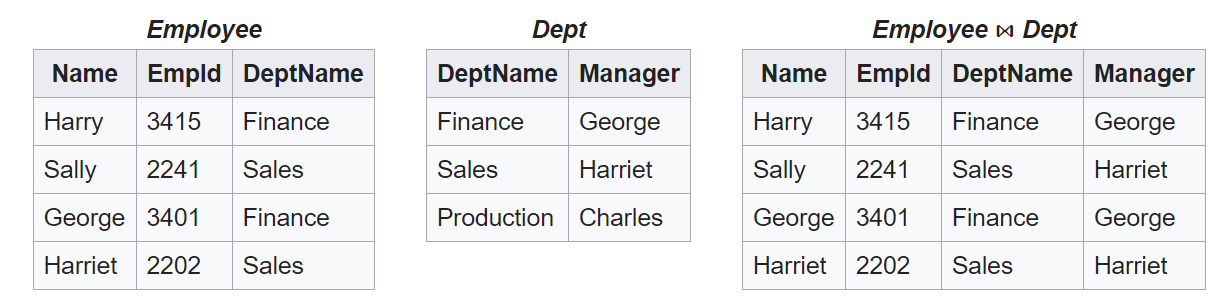
\includegraphics[width=0.5\linewidth]{naturaljoin.png}}
\caption{Examples of natural join}
\label{Natural join example}
\end{figure}

\subsection{Source, target, domain, range}
For binary relations $R \subseteq A \times B$: A is called the \textit{source} and B is called the \textit{target}. Note that source and target are not uniquely determined as:
\[
    Y \supseteq A \quad X \supseteq B
\]

\[
    A \times B \subseteq X \times Y 
\]

\[
    R \subseteq A \times B \subseteq X \times Y
\]

By contrast the \textit{domain}, $dom(R) = \{a : (a,b) \in R \ \textrm{for some } \ b\}$, and the \textit{range}, $range(R) = \{b : (a,b) \in R \ \textrm{for some} \ a\}$


\subsection{Converse and complement}
For a binary relation $R \subseteq A \times B$ its \textit{converse (inverse)} is the relation: $R^{-1} = \{(b,a) : aRb\}$. That is, the relation but with $a$ and $b$ swapped.

\begin{figure}[H]
\center{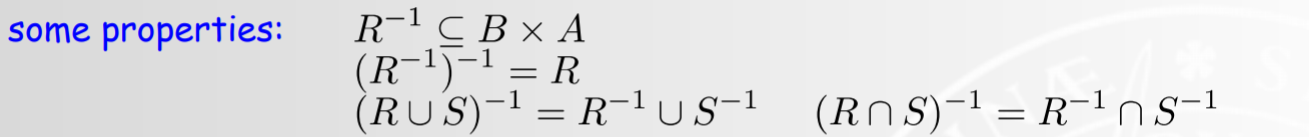
\includegraphics[width=0.5\linewidth]{converse.png}}
\caption{Some properties of the converse of a relation}
\label{Converse properties}
\end{figure}

FOr a binary relation $R \subseteq A \times B$ its \textit{complement} is the relation $\bar{R} = -_{A \times B}R = A \times B \setminus R$. That is, everyting in the cartesian product except the relation itself.

\begin{figure}[H]
\center{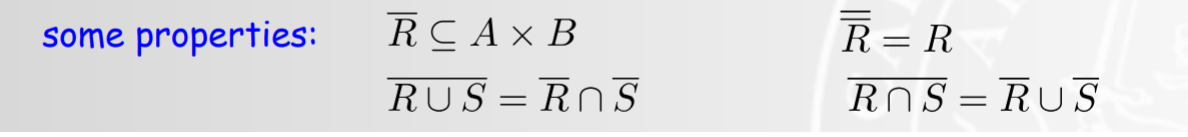
\includegraphics[width=0.5\linewidth]{complement.png}}
\caption{Some properties of the complement of a relation}
\label{Conplement properties}
\end{figure}

\begin{figure}[H]
\center{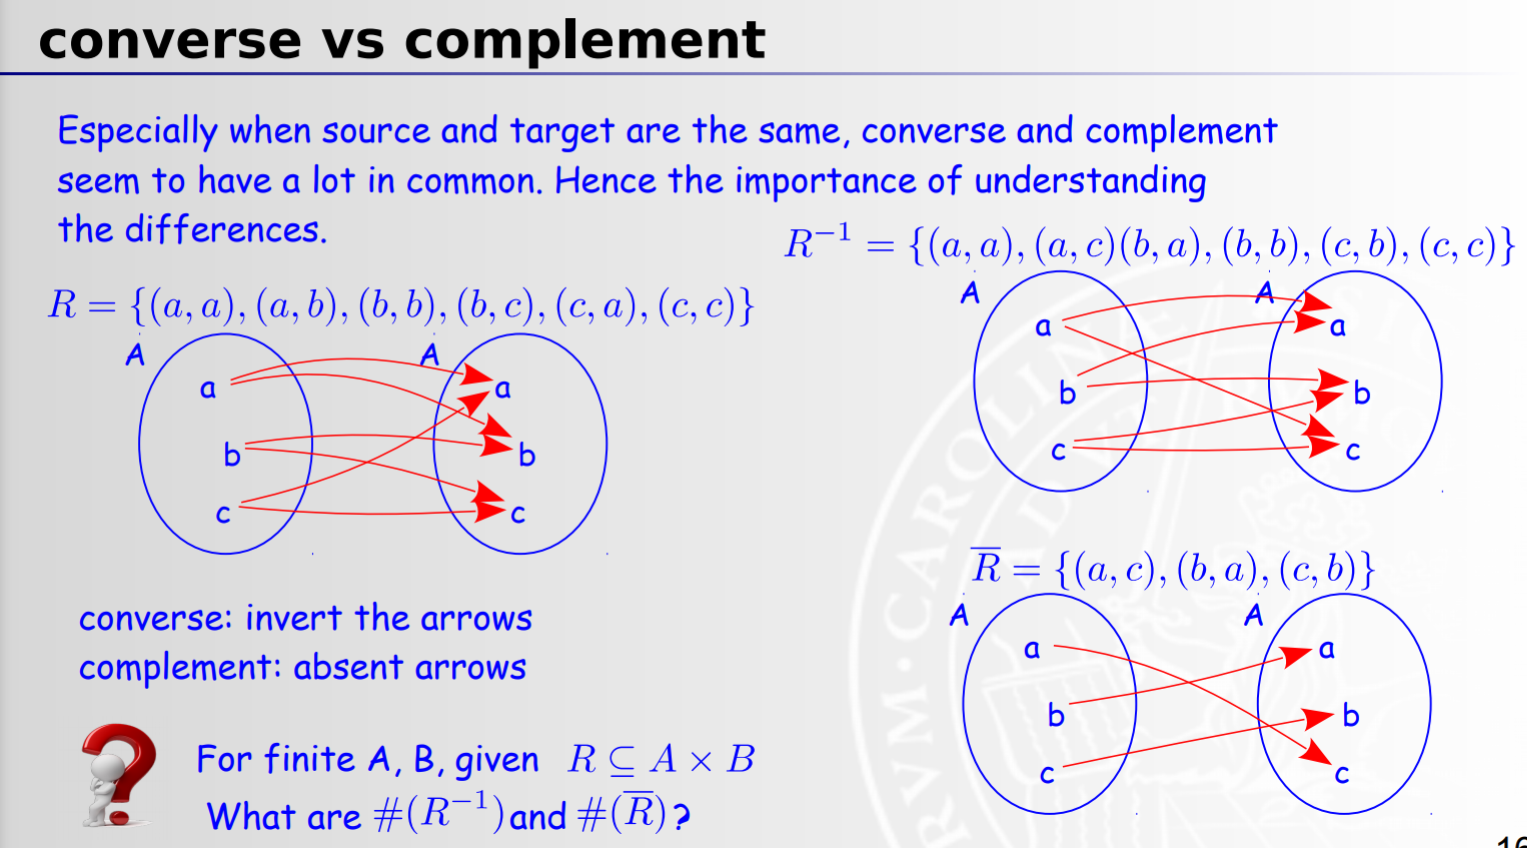
\includegraphics[width=0.5\linewidth]{cvc.png}}
\caption{Converse vs complement}
\label{Converse vs complement}
\end{figure}

\subsection{Composistion}
Given two binary relations $R \subset A \times B$ and $S \subset B \times C$ their \textit{composition} is a binary relation on $A \times C$, or more precise: $S \circ R = \{(a,c) : aRb$ and $bSc$ for some $b \in B\}$ 


\begin{figure}[H]
\center{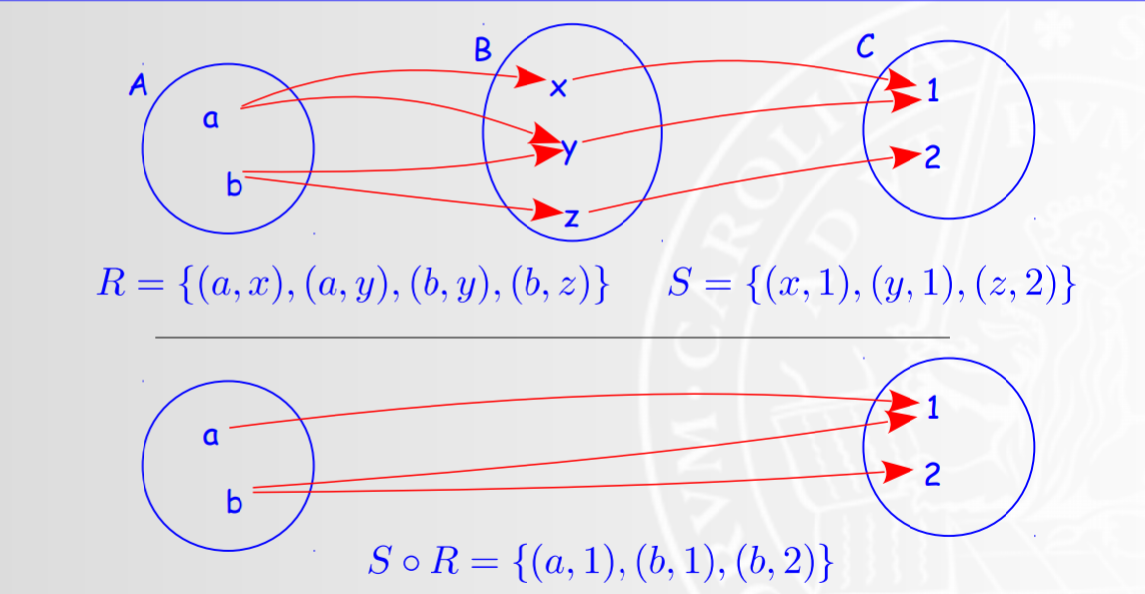
\includegraphics[width=0.5\linewidth]{composition.png}}
\caption{Composition visualised}
\label{Composition visualised}
\end{figure}



\end{document}